
\section{Regime con specifici segnali di ingresso}
\subsubsection{Ingresso esponenziale}
Si ha il segnale in ingresso
$$
u(t) = e^{\lambda t}\qquad \lambda\in\mathbb{C}
$$
La risposta a regime, se esiste è pari a
$$
y_r(t) = \int_0^{+\infty} W(\zeta) e^{\lambda(t-\zeta)} d\zeta = e^{\lambda t}
\int_0^{+\infty} W(\zeta)e^{-\lambda \zeta}
d\zeta
$$
l'integrale ottenuto è proprio la trasformata di Laplace della risposta
all'impulso $W(t)$ calcolata in $\lambda$. Per un sistema asintoticamente
stabile in forma minima, se l'ingresso è un esponenziale, l'uscita sarà
$$
y_r(t) = e^{\lambda t} W(\lambda)
$$
con $\lambda \neq \lambda_i$ autovalori della matrice della dinamica.
$W(\lambda)$ è dunque una costante, una funzione razionale fratta valutata in
$\lambda$, di conseguenza l'uscita sarà pari all'ingresso scalato per la
suddetta costante.
Questa condizione è verificata quasi sempre, ossia le risposte tendono a
seguire gli ingressi a regime.

Se $\lambda$ fosse però pari proprio ad uno zero della funzione di
trasferimento allora l'uscita sarebbe nulla per ogni istante di tempo.
Si dice che gli zeri reali hanno una proprietà \textit{bloccante} per gli
ingressi esponenziali.

\subsubsection{Ingresso sinusoidale}
Sia l'ingresso sinusoidale, sfruttando l'identità di Eulero e la linearità del
sistema, combinate al risultato precedentemente ottenuto per la funzione
esponenziale, si ha:
\begin{equation}
u(t) = \sin(\omega t) \stackrel{\text{Eulero}}{=} \frac{e^{j\omega
t}-e^{-j\omega t}}{2j}\stackrel{\text{Linearità}}{\longrightarrow} y_r(t) =
\frac{W(j\omega)e^{j\omega t} - W(-j\omega)e^{-j\omega t}}{2j}
\label{eq:risposta_sinusoidale}
\end{equation}
Va verificata l'esistenza delle funzioni di trasferimento, l'ascissa di
convergenza coincide con la singolarità polare a parte reale massima ma il
sistema è supposto asintoticamente stabile, di conseguenza tutti gli autovalori
avranno parte reale negativa, il semipiano di convergenza conterrà sicuramente
l'asse immaginario.

Si analizza la funzione di trasferimento valutata in $j\omega$ sfruttando la
definizione di trasformata di Laplace e ancora una volta la formula di Eulero:
$$
W(j\omega) = \int_0^{+\infty} W(t) e^{-j\omega t} dt = \int_0^{+\infty} W(t)
\left(\cos(\omega t) - j\sin(\omega t) \right)dt
$$
Dall'integrale si ottiene che
$$\left.\begin{aligned}
&\Re[W(j\omega)] \qquad \text{è pari}\\
&\Im[W(j\omega)] \qquad \text{è dispari}
\end{aligned}\right\}
\Rightarrow\left\{\begin{aligned}
&|W(j\omega)| \qquad \text{è pari} \\
&\phase{W(j\omega)}\qquad \text{è dispari}
\end{aligned}\right. \Rightarrow
W(-j\omega) = W^*(j\omega)
$$

Si rielabora il risultato \ref{eq:risposta_sinusoidale} con la proprietà appena
ottenuta.
$$\begin{aligned}
y_r(t) &= \frac{|W(j\omega)|e^{j\angle{(W(j\omega))}}e^{j\omega t}
- |W(j\omega)|e^{-j\angle({W(j\omega)})}e^{-j\omega t}  }
{2j} =\\
&=
|W(j\omega)|\frac{e^{j(\omega t + \angle(W(j\omega)))} - e^{-j(\omega t +
\angle(W(j\omega)))}}
{2j} = \\
&= |W(j\omega)|\sin\left(\omega t + \phase{W(j\omega)}\right)
\end{aligned}$$

Si riassume il risultato nel \textbf{Teorema della risposta armonica}
$$
u(t) = A\sin(\omega t + \varphi) \longrightarrow y_r(t) =
A|W(j\omega)|\sin\left( \omega t + \phase{W(j\omega)} + \varphi \right)
$$
Per un sistema asintoticamente stabile in forma minima, la risposta a regime di
un ingresso sinusoidale è ancora una sinusoide alla stessa frequenza di quella
in ingresso, amplificata o attenuata di una quantità pari al modulo della
restrizione all'asse immaginario della funzione di trasferimento, sfasata
inoltre di una quantità pari all'argomento della funzione $W(j\omega)$.

La funzione di trasferimento ristretta all'asse immaginario prende il nome di
\textit{risposta armonica} del sistema
$$
W(j\omega) = \left.W(s)\right|_{s=j\omega} = C(j\omega I-A)^{-1}B + D
$$
dà informazioni sul comportamento in frequenza del sistema, ampiezza e fase
dell'uscita dipenderanno dalla specifica frequenza in ingresso.

Potrebbe accadere che l'armonica in uscita sia esattamente nulla, quando
$j\omega$ è uno zero della funzione di trasferimento, in realtà due zeri
complessi e coniugati sull'asse immaginario.
Essendo la funzione $W(j\omega)$ una funzione regolare, l'intorno degli zeri
viene comunque attenuato dal sistema.

\newpage
\section{Risposta transitoria}
Si definisce come risposta transitoria la differenza nel tempo tra la risposta
del sistema e la risposta a regime.
$$
y_t(t) \stackrel{\text{def}}{=} y(t) - y_r(t)
$$
\begin{figure}[h]
 \centering
 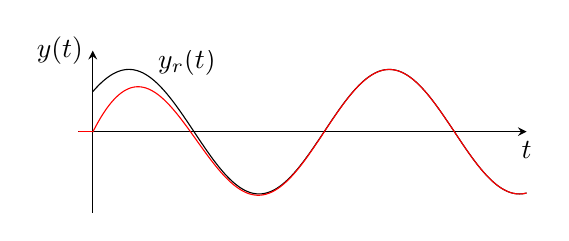
\begin{tikzpicture}
  \begin{axis}[
   width = 0.6\linewidth,
   height=0.3\linewidth,
   axis lines = middle,
   ylabel={$y(t)$},
   xlabel={$t$},
   xtick={0},
   xticklabels={},
   ytick={0},
yticklabels={1},
domain=0:3,
   %x tick label style={yshift=1.5em},
   xlabel style={at={(ticklabel* cs:1)},anchor=north},
   ylabel style={at={(ticklabel* cs:1)},anchor= east},
   ymax=1.3,
   ymin=-1.3,
   xmin=-0.1,
   xmax=3,
   ]
   \addplot[samples=300]{sin(200*(x+0.2))} node[pos=0.11,
above,xshift = 1em]{$y_r(t)$};
   \addplot[samples=300,color=red,width=0.2mm]{-0.65*exp(-3*x) +
sin(200*(x+0.2))};
\draw[color=red,line width = 0.2mm](-0.1,0)--(0,0);
  \end{axis}

 \end{tikzpicture}

\end{figure}
Dall'istante iniziale il sistema impiega un certo tempo per raggiungere la
risposta di regime a partire dalle condizioni iniziali, in questo esempio
parte a riposo, dunque si può affermare che la soluzione complessiva
dell'uscita è somma di due contributi, la risposta transitoria, che si estingue
dopo un certo periodo in un sistema stabile e la risposta a regime.
$$
y(t) = y_t(t) + y_r(t)
$$

Nelle formule di Lagrange sono state definite la \textit{risposta libera} e la
\textit{risposta forzata}, queste non coincidono necessariamente con la
risposta transitoria e la risposta a regime, la risposta transitoria potrebbe
infatti contribuire sia all'evoluzione libera che a quella forzata.

Si considera ad esempio un ingresso esponenziale
$$
u(t) = e^{\lambda t} U \longrightarrow U(s) = \frac{U}{s-\lambda}
$$
La risposta completa sarà l'antitrasformata delle evoluzioni libere e forzate
$$
y(t) = \Lap^{-1} \left[ \Psi(s)x_0 + W(s)\frac{U}{s-\lambda}  \right]
$$
Analizzando la forzata, si esegue la scomposizione in residui aggiungendo il
fratto relativo all'ingresso $R_u$
$$
y_f(t) = \Lap^{-1}\left[\sum_i \frac{R_i}{s-\lambda_i} +
\frac{R_u}{s-\lambda}\right]
$$
La sommatoria fornirà un termine chiamato $y_1(t)$ e il residuo $R_u$ una
funzione $y_2(t)$, per ipotesi i $\lambda_i$ hanno parte reale negativa, quindi
tutti i termini della funzione $y_1(t)$ tendono a zero.
Di conseguenza il regime è proprio la seconda parte dell'equazione,
$y_2(t)=y_r(t)$, quella parte della forzata che dipende dalle singolarità
polari dell'ingresso, per questo motivo ha la stessa forma dell'ingresso,
cambiando il residuo $R_u$ che dipende dal sistema cambieranno ampiezza e fase.

La somma di $\Lap^{-1}[\Psi(s)x_0]=y_l(t)$ e $y_1(t)$ forma il transitorio
$y_t(t)$.
Il regime esiste se non dipende dallo stato iniziale $x_0$, in realtà è il
transitorio $y_t(0)$ che deve estinguersi a zero. Potrebbe teoricamente
capitare che il transitorio tenda a zero perché $y_l(t)$ e $y_1(t)$ siano
istante per istante uguali e opposte.
Questo fenomeno può in realtà accadere solo per ingressi esponenziali o
combinazioni di esponenziali (es. sinusoide).
Si rimuove l'ipotesi di asintotica stabilità.

Esempio:
$$
u(t) = Ue^{\lambda t} \longrightarrow y(t) \propto e^{\lambda t}
$$
Dato che l'uscita segue l'ingresso, e l'uscita dipende dallo stato, anche lo
stato dovrà avere una forma esponenziale. Si supponga che sia della seguente
forma:
$$
x(t) = e^{\lambda t}x(0)
\stackrel{\dot{x}=Ax+Bu}{\longrightarrow}\lambda \cancel{e^{\lambda t}}x(0) =
A\cancel{e^{\lambda t}}x(0) + BU\cancel{e^{\lambda t}} \Rightarrow (\lambda
I-A)x(0) = BU
$$
Si suppone che $\lambda \neq \lambda_i$, la matrice $(\lambda I -A)$ è
invertibile dunque la soluzione esiste ed è unica
$$
x(0) = (\lambda I -A)^{-1}BU
$$
se lo stato iniziale è esattamente questo, la risposta transitoria sarà
identicamente nulla $\forall t$ anche senza ipotesi di asintotica stabilità.
$$\begin{aligned}
x(t)  &= (\lambda I -A )^{-1}BUe^{\lambda t} &  & t\geq 0\\
y(t) &= Cx(t) +Du(t) = \left(C(\lambda I-A)^{-1}B+D\right)Ue^{\lambda t}
=W(\lambda)Ue^{\lambda t}
&  &
t\geq 0
\end{aligned}$$
Quanto ottenuto è solo un risultato puramente matematico, se un sistema non è
asintoticamente stabile non ammetterà un regime permanente.

\newpage
\section{Identificazione sperimentale della risposta armonica}
Si supponga di avere un sistema da studiare di cui si conoscono gli ingressi e
le uscite, non si conoscono le caratteristiche interne del sistema a causa
della inaccessibilità del sistema stesso o all'impossibilità di realizzarne un
modello accurato.
È possibile caratterizzare il sistema valutando la \textbf{risposta in
frequenza}, si applica al sistema una sinusoide
$$
u(t)  = U\sin(\omega t)
$$
Si vede se dopo un certo tempo l'uscita sia ancora una funzione sinusoidale
alla stessa frequenza dell'ingresso, il sistema avrà un comportamento lineare
a quella specifica frequenza
$$
y_r(t) = U|W(j \omega)|\sin(\omega t + \phase{W(j \omega)})
$$
Si misura il rapporto tra ampiezza di ingresso e uscita e si riporta su un
grafico funzione della frequenza, analogamente l'angolo.

Si varia successivamente la frequenza, all'estinguersi del transitorio si
misurano nuovamente ampiezza e frequenza e così via per più frequenze.
Si può valutare anche a frequenza nulla (guadagno statico).
\begin{figure}[h]
 \centering
 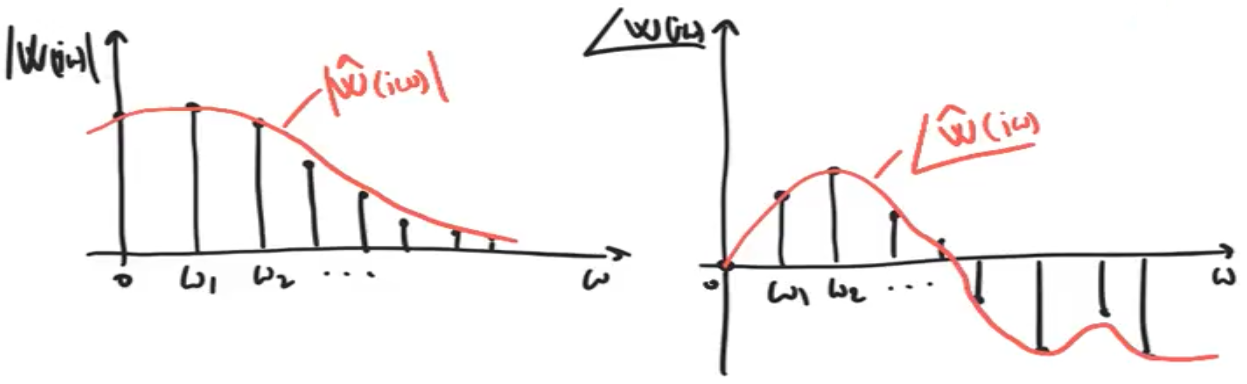
\includegraphics[width=0.6\linewidth]{ricostruzione_risposta_in_frequenza}
\end{figure}

Si scelgono le funzioni interpolanti delle curve ottenute
$$
|\hat{W}(j\omega)| \qquad \phase{\hat{W}(j\omega)} \Rightarrow \hat{W}(j\omega)
$$
Si è ricostruita sperimentalmente la funzione di risposta armonica.

La $W(s)$ è una funzione razionale fratta, dunque analitica, se si definisce
una funzione analitica in un sottoinsieme non numerabile $s$ allora si può
estendere la definizione a tutto lo spazio rimanente.
Se la funzione $W(j\omega)$ che è una funzione analitica, è definita sull'asse
immaginario, che è uno spazio non numerabile, si può estendere la definizione a
tutto lo spazio, ottenendo una stima della funzione di trasferimento del
sistema sostituendo $s$ a $j\omega$, si ottiene un modello sperimentale
approssimato del sistema.

Solitamente un modello approssimato mediante un'analisi sperimentale può
essere di ordine più alto dell'ordine reale del sistema, si perdono inoltre
informazioni sulle relazioni fisiche del sistema.

Un modello sperimentale potrebbe comunque essere più accurato di un modello
costruito analiticamente utilizzando i dati di targa del sistema, con la loro
soglia di incertezza che non corrispondono necessariamente alla realtà, un
modello sperimentale potrebbe invece approssimare meglio i punti reali
raggiunti dal sistema.

Per analizzare l'intero spettro in frequenza del sistema bisognerebbe
sollecitare il sistema di volta in volta con un'armonica differente, oppure
si può usare direttamente un segnale che contiene più armoniche come ad esempio
il gradino che le contiene tutte.
Si misura l'uscita e con un analizzatore di spettro si analizzano le frequenze
in uscita dal sistema ottenendo facilmente informazioni sul comportamento del
sistema ad un gran numero di armoniche.

\section{Analisi con ingresso periodico}
Sia il segnale periodico
$$
u(t)\ \ T\text{ periodico} \Leftrightarrow u(t+T) = u(t)
$$
è sviluppabile in \textit{serie di Fourier}
$$
u(t) = \sum_{n=-\infty}^{+\infty} U_n e^{j\omega t}
$$
con $U_n$ i coefficienti di Fourier e $\omega = \frac{2\pi}{T}$.
La serie dei coefficienti di Fourier definisce lo spettro del segnale in
ingresso, che avrà un'infinità numerabile di coefficienti.

L'uscita a regime $y_r(t)$ esisterà per la linearità del sistema e sarà pari
alla stessa combinazione lineare dell'ingresso
$$
y_r(t) = \sum_{-\infty}^{+\infty} U_nW(jn\omega)e^{j\omega t} =
\sum_{-\infty}^{+\infty}Y_n e^{j n \omega t}
$$
L'uscita ha la forma dello sviluppo in serie di Fourier di un segnale, dunque
si può affermare che il segnale in uscita è periodico.
Il peso dei coefficienti sarà differente dunque il segnale in uscita sarà
comunque deformato rispetto a quello in ingresso.

Si supponga che il segnale in ingresso sia dotato di trasformata di
Fourier $U(j\omega)$, se ciò è vero esiste ed è finito il seguente integrale
$$
u(t) = \frac{1}{2\pi}\int_{-\infty}^{+\infty} U(j\omega)e^{j\omega t}d\omega
$$
La trasformata è bilaterale, non è richiesto che il segnale sia nullo per
$t<0$, sfruttando la linearità del sistema e dell'integrale si ha l'uscita a
regime
$$
y_r(t) = \frac{1}{2\pi}\int_{-\infty}^{+\infty} U(j\omega) W(j\omega)
e^{j\omega t} d\omega = \frac{1}{2\pi}\int_{-\infty}^{+\infty} Y(j\omega)
e^{j\omega t} d\omega
$$
Si è ottenuta l'antitrasformata di Fourier di $Y(j\omega)$ che sarà dunque lo
spettro del segnale in uscita, può contenere al più le armoniche del segnale
d'ingresso, potranno essere attenuate o amplificate dalla funzione
$W(j\omega)$, se la banda del segnale in ingresso è limitata entro certe
frequenze, anche l'uscita sarà limitata in quella banda.

Ancora una volta, nell'ipotesi di sistema SISO, la funzione di risposta
armonica si ottiene analogamente alla funzione di trasferimento $W(s)$ nel
dominio di Laplace:
$$
W(j\omega) = \frac{Y(j\omega)}{U(j\omega)}
\qquad \begin{aligned}&j\omega \rightarrow s\\
&s\leftarrow j\omega
\end{aligned}\qquad W(s) =
\frac{Y(s)}{U(s)}
$$
